\documentclass{article} % For LaTeX2e
\usepackage{amstext}
\usepackage{amsmath}
\usepackage{iclr2018_conference,times}
\usepackage{hyperref}
\usepackage{url}
\usepackage{txfonts}
\usepackage{pxfonts}
\usepackage{graphicx}
\usepackage{etoolbox}
\AtBeginEnvironment{quote}{\small}

\begin{document}

\title{Vacuum Cleaners: The Bleeding Edge of AI}

\author{Lawrence Neal and Matthew Olson}

\newcommand{\fix}{\marginpar{FIX}}
\newcommand{\new}{\marginpar{NEW}}

\iclrfinalcopy % Uncomment for camera-ready version, but NOT for submission.

\maketitle

\begin{abstract}
    In order to test different AI agent implementations, we create simulated vacuum cleaning environments. We test 3 different AI types and measure their ability to clean quickly and fully: finding an agent with state performing well in some instances and that a stochastic agent performs well in other environments.
\end{abstract}

\section{Introduction}

\begin{figure}[h]
\begin{center}
    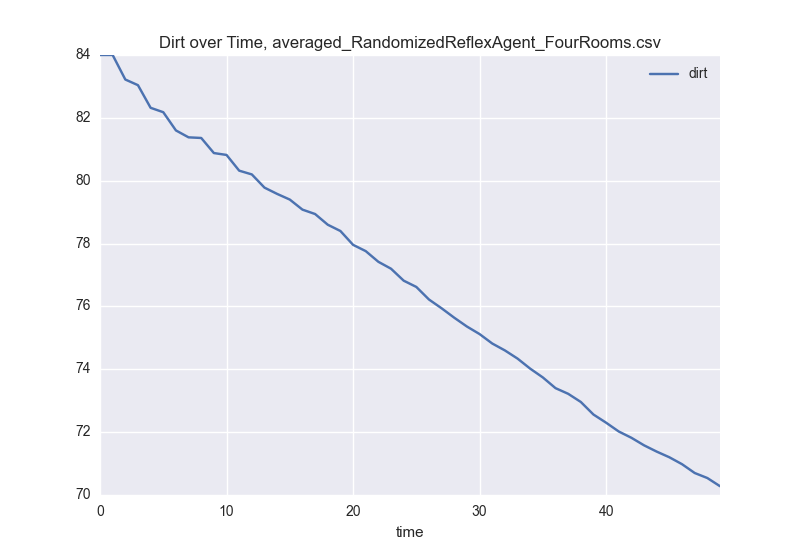
\includegraphics[width=\linewidth]{fig_001.png}
\end{center}
\caption{image include test}
\end{figure}

things go here

\section{Methods}


Every agent is designed such that it will suck if the dirt percept is true.
First agent is the simple reflex agent. It will move forward one square at a time until it the “wall” flag is true in its percepts. When it sees a wall, it will turn left.
2nd agent is the randomized reflex agent. We designed it so that it will act the same at the previous agent. Moving forward when there is no wall in front of it. We also added a the ability for it to stochastically decide whether to turn left or right when it sees a wall with equal probability. If there is no wall it will randomly choose between turning right and moving forward. We split this agent into 3 sub agents: changing the probability of selecting turning over moving forward. We ended choosing 10\%, 20\% and 30\% for the different p values.
The last agent is the Deterministic Model Based Reflex Agent. The idea behind it is to make an incremental sweeping pattern. It will move forward until it hits a wall, but instead of simply turning and moving forward again, it will turn, move a space, turn again, and change direction of the next turn sequence. This allows it to traverse the empty room fully. By using state, it can keep track of which direction it is turning, and keep track of knowing if it should be moving forward on when there is no wall, or if it should turn again. This agent follows the included state diagram. Suck actions are omitted as it always sucks when there is dirt regardless of state.
\begin{figure}[h]
\begin{center}
    \includegraphics[width=\linewidth]{state_diagram.png}
\end{center}
\caption{Deterministic Model Based Reflex Agent mov}
\end{figure}

\section{Agent If-Then Statement Descriptions}
Simple Reflex: 
If dirt then suck
If wall then left
Else Forward

RandomReflexAgent:
If dirt then suck
If wall then \(If random50percent then left else right\)
If no wall then \(If randomNum greater than probablity_right then forward else right\)
Else Forward

DeterministicModelBasedReflexAgent:
If dirt then suck
If state == 0 and wall then (right and increment state) 
If state == 0 and no wall then forward
If state == 1 and wall then right 
If state == 1 and no wall then (forward and increment state)
If state == 2 then (right and increment state)
If state == 3 and wall then (left and increment state)
If state == 3 and no wall then forward
If state == 4 and wall then left 
If state == 4 and no wall then (forward and increment state)
If state == 5 then (left and state = 0)


\section{Experiments}
TODO: do we use this section? Maybe just show graphs here
\section{Results}

TODO: put result number in
TODO: put in graphs

\subsection{Simple Reflex Agent}
The best possible performance achievable by the simple reflex agent in the empty room is getting all of the pieces of dirt on the outside where the perimeter of the room is. It cannot clean the room with any dirt on the non-perimeter perfectly as it has no way to get into the center area of the room. When it turns it then immediately forgets that it has turned and continues forward along. If it were to have some sort of memory it would know that it had just turned and could use that to get to the center area.

For the second room the best possible scenario would be having each doorway towards the center of the entire area. If in the first room the doors are on the very top right corner and the other rooms structured similarly, Then the agent could Traverse through the door go around the perimeter of each other room and continue onto the Next Room through the second door. However this one still not be perfect as it will not be able to reach the very center of the individual rooms. It again would require some sort of memory to know that it had turned and needed to turn again to get to the center of the rooms. 

\subsection{Random Agents}

\begin{table}[]
\centering
\caption{Random Agents actions to clean 90 percent of room}
\label{is this label used?}
\begin{tabular}{lll}
     & Empty Room & 4 Rooms \\
p=.1 & 798.40 & 1012.58 \\
p=.2 & 619.36 & 790.04  \\
p=.3 & 641.56 & 866.3  
\end{tabular}
\end{table}

The random agent performs moderately. Is able to clean rooms eventually, but it is quite slow compared to the memory-based deterministic agent. However, that doesn't mean that it is worse, as it does clean a higher percentage of the entire environment than the memory based agent. 
The benefit of including Randomness with an agent is it will take actions that will lead it to discover unexplored areas. The detriment is that it will take actions that cause it to repeat itself and cover already traversed ground. 

\subsection{memory-based deterministic agent}
The memory-based deterministic agent performs very well in the empty room. It is able to make a sweeping pattern across the room and make very little overlap on the already cleaned spaces and cleans the room perfectly.  The performance in the next environment depends on the placement of the doors. There are some placements for the doorways where the agent is unable to find that doorway before leaving the room from the same door entered. That's it will leave some rooms uncleaned. They can also accidentally leave a room too early if it is making its sweeping pattern and runs into the door before finishing. \par

TODO: How long does it take? \par

The agent can definitely be improved with more memory. More memory would enable it to know how large a room is. If it knows how large the room is it can adjust it sweeping pattern such that it will not accidentally take doors. If it had more memory it could know where the placement of the doors are, clean the room, and immediately head for the Next Room.

\section{Conclusion}
There are a couple of trade-offs between the random and deterministic agents. In order for the random agent to attempt to make it to the center of a room it has to randomly decide to turn. By making this turn it may Traverse an already cleaned area thus making it less efficient, however, this enables it to traverse more complex environments because it can randomly turn into doorways that a deterministic agent would have a harder time going through. The reason a deterministic agent with have a harder time making it through these doorways is that through its sweeping patterns it may miss the doorway and have to sweep in the opposing Direction. \par
There are two easy ways to design a better agent for more complicated environment. The first one is to give the agent more percepts. If the agent were able to see walls on the left and right of it, instead of just in front of it, then it could know when a doorway is on the side of it and must be entered. The next way to design agent better is to add more memory. With only two  or 3 bits of memory it is difficult for an agent to know how best to clean the room. \par

\end{document}

